\documentclass[nochap, headernames]{config/ejercicios}

\title{Prácticas Filogenia molecular (PHYLO)}
\author{Sandra Mingo Ramírez}
\date{2024/25}

\usepackage[all]{nowidow}
\usepackage{listing}
\usepackage{color}
\usepackage{tabularx}
\usepackage{multirow}
\usepackage{makecell}
\usepackage{amsmath}
\usepackage{array}
\usepackage{hyperref}

\begin{document}

\maketitle

%Programas adicionales: Genius, Ugene (alternativa gratuita de genius), Phylemon
%SeaView es un programa muy simple que permite arrastrar cualquier archivo para abrir alineamientos o árboles. Permite realizar funciones simples, pero que podrían ser laboriosas en otros programas, como por ejemplo eliminar el nucleótido en la posición X. 

\section{Formatos de archivos  filogenéticos y alineamientos}
El objetivo es familiarizarse con la conversión de formatos de archivo, diferentes métodos de alineación, eliminación de posiciones ambiguamente alineadas, edición de matrices y traducción de secuencias de ADN a proteínas.
\begin{enumerate}
\item Alinea el conjunto de datos utilizando MAFFT (en línea) con la estrategia Auto. Guarda el alineamiento resultante en formato fasta. \footnote{Los archivos fasta empiezan con el símbolo > seguido de un descriptor de la secuencia. Después, empieza la secuencia en una nueva línea. Cuando termine, hay un nuevo prompt con un nuevo descriptor.}
\item Alinea el conjunto de datos utilizando CDS-ProtAl: Utilidades > Utilidades de Alineación > CDS-ProtAl > Examinar servidor > Cargar nuevo archivo, Seleccionar formato > Secuencias no alineadas > Cargar > Aceptar, Parámetros > Mantener huecos, Código genético > Estándar. Ejecutar.
\item Compara las dos alineaciones resultantes utilizando SeaView. Arrastra el archivo de salida MAFFT. Luego Archivo > Nueva Ventana, arrastre el archivo de salida CDS-ProtAl.
\item Utiliza TrimAl para eliminar las posiciones ambiguamente alineadas. Esto puede hacerse automáticamente (redirigiendo el archivo resultante de CDS-ProtAl en Phylemon) o manualmente (Utilidades > Utilidades de Alineación > TrimAl). Selecciona Método 'sin huecos' para este ejercicio.
\item Utiliza SeaView para traducir una matriz de secuencia de nucleótidos a aminoácidos. Utiliza el conjunto de datos de TrimAl. Arrastra el archivo. Props > Ver como proteínas. Archivo > Guardar prot alineación. \textbf{Nota}: Si es necesario, se puede cambiar el código genético: Edit > Set genetic code.
\item Familiarízate con la conversión de formatos de archivo utilizando ALTER. Introduce el archivo de entrada en formato fasta (paneles de la izquierda): 
\begin{enumerate}
\item Seleccionar formato > Autodetectar
\item Cargar o pegar MSA > Seleccionar sistema operativo > Linux / Mac OS X. Seleccione el de salida (paneles derechos): Seleccionar programa > RAxML, formato > PHYLIP, Convertir
\item Guardar MSA convertido > Seleccionar sistema operativo > Linux / Mac OS X, Guardar
\item Repita la exportación al formato Nexus (Seleccione programa > MrBayes, formato > NEXUS).
\end{enumerate}
\end{enumerate}

MAFFT es un programa muy utilizado. Tiene una versión descargable y una versión en línea que permite utilizar los servidores localizados en Japón. La versión en línea cuenta con un cuadro donde pegar los datos, aunque también se puede seleccionar un archivo desde el disco duro. En nuestro caso, subiremos el archivo \texttt{HRSV-A\_modif\_RAW.fas}. Se pueden elegir algunas opciones de estética, como el uso de mayúsculas y minúsculas (la convención es poner los nucleótidos en minúscula y los aminoácidos en mayúscula), la dirección de las secuencias (se le puede pedir al programa que compruebe y ajuste la direccionalidad, aunque consume más recursos y tarda más tiempo) y el orden de la salida. Poner un nombre al trabajo puede ser útil cuando se van a lanzar varios trabajos simultáneamente. También permite poner una dirección de correo que notifique cuando se ha terminado de analizar un trabajo que vaya a tardar mucho para evitar tener que estar con la pestaña del ordenador abierta. Entre la configuración avanzada, se puede seleccionar la estrategia. Los métodos progresivos van alineando las secuencias en parejas y las van alineando poco a poco, añadiendo gaps donde toque según ese alinamiento. Los métodos iterativos, después de alinear todas las secuencias, vuelve al principio a reevaluar el alineamiento y mejorándolo. Por este motivo, los métodos iterativos son más lentos y se recomiendan para sets de pocas secuencias. También hay una estrategia automática que evalúa cuatro de los algoritmos según el tamaño de los datos y utiliza uno u otro. El resultado del alineamiento después de darle al botón de Submit es el que aparece en la imagen \ref{fig:mafft-result}.

\begin{figure}
\centering
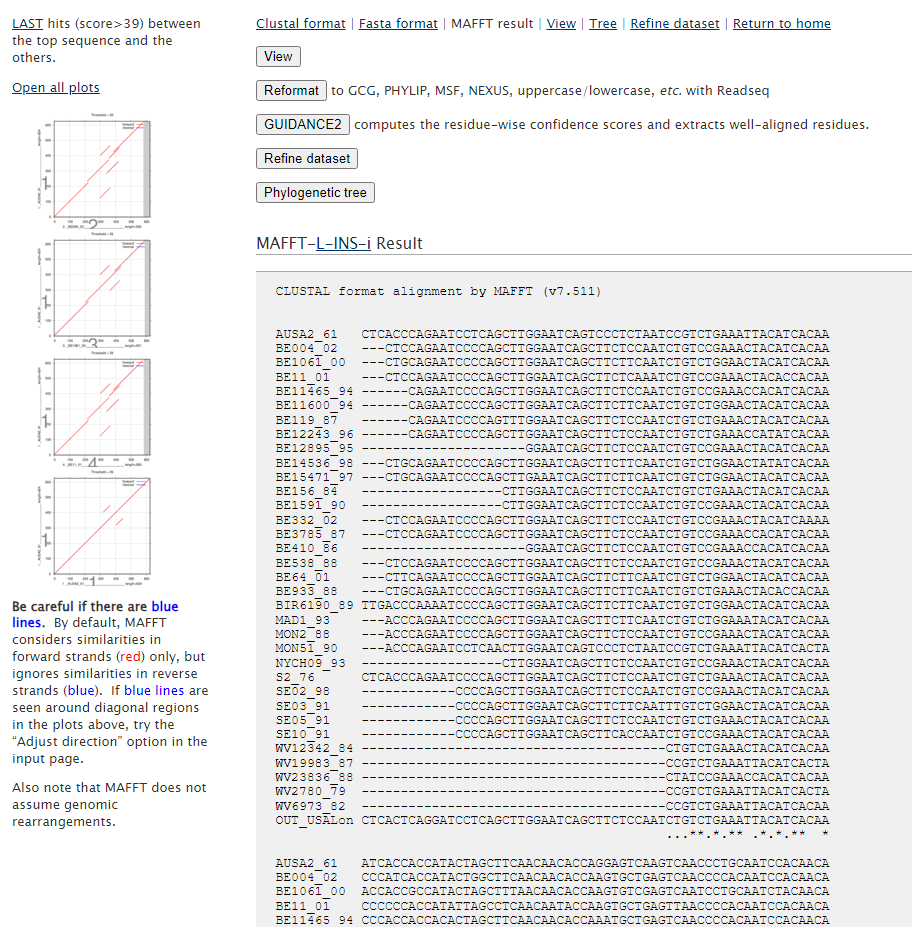
\includegraphics[width = \linewidth]{figs/mafft-result.png}
\caption{Resultado del alineamiento del fichero HRSV-A. La parte de la izquierda muestra unos gráficos de similitud. Debería estar todo en rojo, ya que si hay alguna línea en azul, eso indicaría que hay secuencias invertidas y que habría que reevaluar el alineamiento ajustando la direccionalidad.}
\label{fig:mafft-result}
\end{figure}

Para guardar el alineamiento, lo más cómodo es pulsar el botón de \texttt{Fasta format} en la parte superior. Este alineamiento lo podemos visualizar entonces en el programa de SeaView o en \href{http://phylemon.bioinfo.cipf.es/}{Phylemon}. \footnote{Tradicionalmente funcionaba bien en Google Chrome y daba error o no cargaba en otros navegadores. Ahora parece ser que es al revés; no carga usando Google Chrome, pero en Firefox funciona bien.} Este último tiene en el cluster programas de terceros para realizar alineamientos, árboles filogenéticos, test evolutivos y pipelines para combinarlos, pero también otras utilidades exclusivas. Dentro de las utilidades de alineamientos, hay tres programas: ConcatenAl permite concatenar los alineamientos, CDS-ProtAl sirve para traducir proteínas desde las secuencias codificantes, y TrimAl permite eliminar partes de la secuencia que están alineadas de forma dudosa o que tienen gaps. Nosotros vamos a utilizar CDS-ProtAl, donde podemos pegar una secuencia o subirla. Al subir un archivo, hay que seleccionarlo y decir el tipo de archivo que es (secuencia alineada, sin alinar, árbol, etc). Los parámetros que se pueden seleccionar son mantener o no los gaps y traducir la secuencia sin alinearla. También pide el código genético para poder traducir las proteínas. En nuestro caso del virus respiratorio sincitial humano, utilizaremos el código genético estándar. Una vez terminado el trabajo, nos podemos descargar los ficheros resultantes pulsando sobre el nombre o haciendo click derecho y "guardar enlace como". Aunque el formato sea out\_ali, se puede cambiar manualmente a fasta y visualizar con SeaView. 

Hay algunos casos en los que las regiones no alineadas pueden producir mucho ruido filogenético. Para eso, existen programas que permiten seleccionar bloques de secuencia conservada, como Gblocks o TrimAl. Desde Phylemon, se puede redirigir el resultado obtenido con CDS-ProtAl directamente a TrimAl (y otras herramientas) mediante un desplegable, facilitando así el trabajo y evitando tener que descargar los archivos intermedios y temporales. Antes de lanzar el trabajo con TrimAl, permite seleccionar la eliminación de secuencias de baja similitud o calidad antes de quitar las posiciones. Hay varios métodos para quitar los gaps: "no gaps" quita todas las posiciones que tengan un gap,"no all gaps" quita las posiciones que sólo sean gaps y no tengan ninguna secuencia, y "gappyout" quita las posiciones que tienen más gaps de lo esperado. 

Desde SeaView se puede también traducir una secuencia a proteínas mediante Props y el check de "ver como proteínas". En "File" se puede guardar el archivo. En algunos casos, algunas posiciones son muy variables (por ejemplo, las terceras posiciones de los genes mitocondriales, que tienen tantos cambios superimpuestos que no aportan información filogenética), por lo que es mejor eliminar las posiciones antes de realizar los análisis. En SeaView, esto se puede hacer en Sites y Create Set. A continuación se puede seleccionar aquellas posiciones que se quieren. Por ejemplo, para eliminar las terceras posiciones, habría que utilizar la opción que selecciona la primera y segunda posición. Para guardar esta selección, en File hay una opción de Save selection.
\section{Máxima parsimonia y visualización de árboles}
El objetivo de esta práctica es obtener árboles filogenéticos utilizando la máxima parsimonia utilizando un alineamiento de secuencias de ADN múltiple y visualizar los árboles con un visualizador gráfico. Los pasos para hacer esto en el programa de Mega son:
\begin{enumerate}
\item Abrir el archivo en File > Open a File/Session > Analyze. Selecciona el tipo de datos de acuerdo a su naturaleza, es decir, si se trata de nucleótidos, proteínas, si es codificante o no codificante, etc.
\item Construye el árbol en Phylogeny > Construct/Test Maximum Parsimony Tree(s). Hay varios campos con el borde resaltado que se pueden modificar:
\begin{itemize}
\item Test of Phylogeny: Sólo podemos hacer una búsqueda del árbol de máxima parsimonia, o también podemos hacer un análisis bootstrap. Si hacemos bootstrap, deberíamos hacer 1000 réplicas bootstrap, pero, dadas las limitaciones de tiempo, haremos 100 réplicas para este ejercicio.
\item Substitution Type: nucleótido o aminoácido si la secuencia de nucleótidos se ha marcado como codificante. Seleccionar aminoácidos aquí tendría el mismo efecto que eliminar la tercera posición de los análisis. 
\item Gaps/Missing Data Treatment: utiliza todos los sitios
\item Select Codon Positions: Prueba con varios árboles utilizando todas las posiciones, solo la primera y segunda posición, o solo la tercera posición.
\item MP Search Method: Tree-Bisection-Reconnection (TBR)
\item No. of initial trees (random addition): 10
\item MP Search level: 1
\item Max No. of trees to retain: 100
\item Compute (OK)
\end{itemize}
\item El árbol aparece en una nueva ventana. Si es necesario, se puede volver a enraizar en Subtree > Root.
\item Guardar el árbol desde File > Export Current Tree (Newick). Esto abre una ventana que se debe guardar pulsando en el botón del disquete o copiando y pegando en un documento de texto. El árbol se puede abrir y visualizar en un visualizador gráfico de árboles filogenéticos, como FigTree.
\end{enumerate}

El formato Newick utiliza los paréntesis para mostrar la jerarquía de los taxones en un árbol filogenético. También puede incluir las longitudes de las ramas o los valores de soporte del bootstrap. En ese caso, se utilizan los dos puntos con los taxones o con la relación (el paréntesis) respectivamente. 

FigTree está diseñado como visor gráfico de árboles filogenéticos y como programa para producir figuras listas para su publicación. Para visualizar el árbol con FigTree se realiza de la siguiente forma:
\begin{enumerate}
\item Abre el archivo del árbol (formato Newick o Nexus) en FigTree. Si el árbol está anotado (por ejemplo con valores adicionales en ramas/nodos), aparecerá una ventana solicitando un nombre específico para las anotaciones que el árbol tiene asociadas a sus nodos. En nuestro caso, se trata de los valores de soporte bootstrap, por lo que les daremos un nombre (por ejemplo, soporte).
\item Explora las opciones de enraizado, opciones de visualización y de ramas/nodos. Las distintas opciones se pueden seleccionar utilizando los paneles superiores o izquierdos. 
\end{enumerate}

Se puede cambiar el tamaño de la letra de los taxones desde Tip Labels > Font Size. También se puede enraizar un árbol desde FigTree, pulsando en una rama y en el botón de Reroot. Se pueden ordenar los nodos de forma ascendente o descendente desde Trees > Order nodes > Ordering y colorear las ramas en función de su valor de soporte. 

\begin{figure}[htbp]
\centering
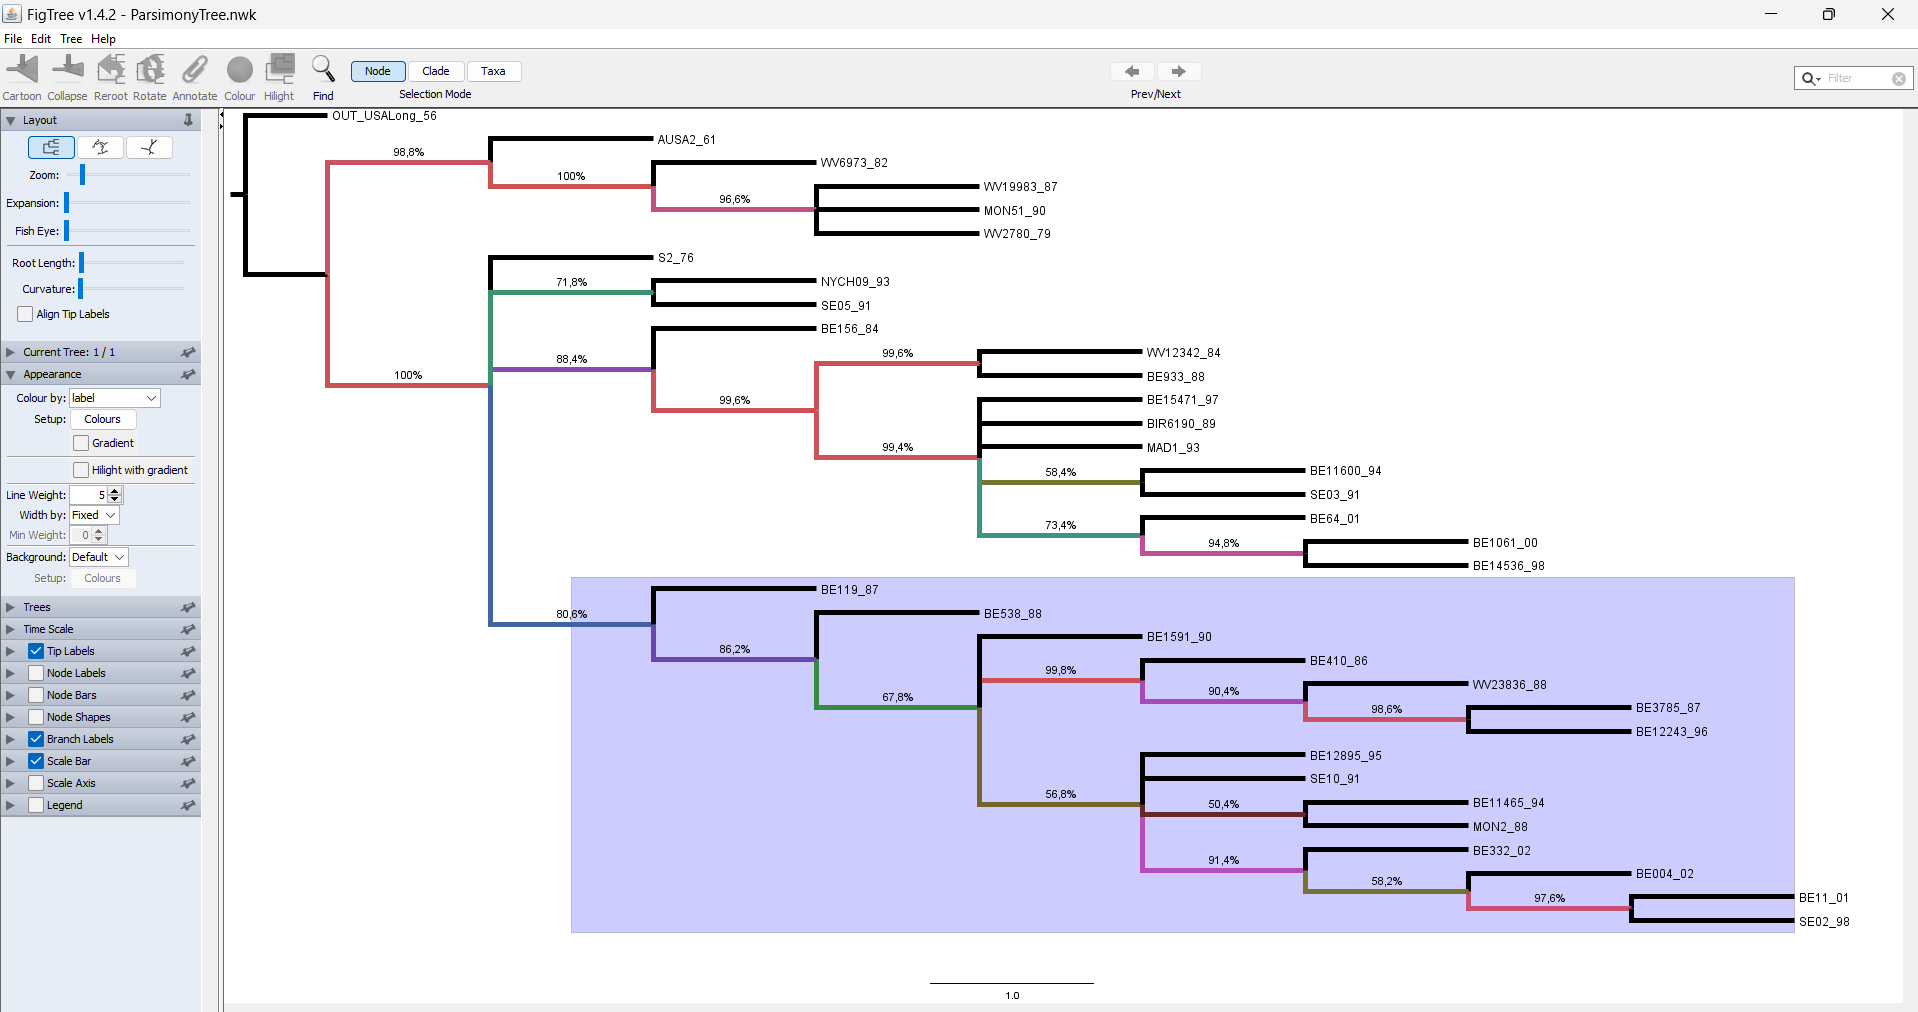
\includegraphics[width = \linewidth]{figs/figtree.png}
\end{figure}

Una de las plataformas para hacer árboles utilizando la máxima parsimonia es \href{https://www.lillo.org.ar/phylogeny/tnt/}{TNT}. El problema es que, pese a ser muy potente, es muy complicado de utilizar.
\section{Modelos de evolución}
El objetivo de esta práctica está en seleccionar el mejor modelo de sustitución para distintos tipos de datos: nucleótidos y aminoácidos. Para seleccionar el \textbf{mejor modelo de sustitución de nucleótidos} desde el servidor de IQ-Tree se deben realizar los siguientes pasos:
\begin{enumerate}
\item Ve al \href{http://iqtree.cibiv.univie.ac.at/}{servidor de la web de IQ-Tree}.
\item Cambia a la pestaña de Selección de Modelos.
\item Carga el fichero del alineamiento de nucleótidos.
\item Selecciona el tipo de secuencia (en este caso ADN) o déjalo como detección automática.
\item Cambia los criterios de selección a AIC para este ejercicio.
\item No cambies ninguna otra opción.
\item Opcional: deja un correo electrónico para poder obtener los resultados directamente.
\item Pulsa a submit job.
\item Una vez terminado, comprueba los resultados en la ventada de Full Results. Descarga los resultados y examina los distintos archivos en editores de texto plano.
\end{enumerate}

Para seleccionar el \textbf{mejor modelo de sustitución de aminoácidos} desde el servidor de IQ-Tree se deben realizar los siguientes pasos:
\begin{enumerate}
\item Ve al \href{http://iqtree.cibiv.univie.ac.at/}{servidor de la web de IQ-Tree}.
\item Cambia a la pestaña de Selección de Modelos.
\item Carga el fichero del alineamiento de nucleótidos.
\item Selecciona el tipo de secuencia DNA -> AA, carga el alineamiento de aminoácidos y selecciona Protein o déjalo como detección automática.
\item Elige el código genético apropiado (en este caso, estándar o universal).
\item Cambia los criterios de selección a AIC para este ejercicio.
\item No cambies ninguna otra opción.
\item Opcional: deja un correo electrónico para poder obtener los resultados directamente.
\item Pulsa a submit job.
\item Una vez terminado, comprueba los resultados en la ventada de Full Results. Descarga los resultados y examina los distintos archivos en editores de texto plano.
\end{enumerate}

Si sabemos que nuestros datos son ADN o aminoácidos, es mejor indicar en IQ-Tree el tipo de secuencia que no dejar que lo detecte de forma automática. Esto se debe a que las letras de los nucleótidos también se utilizan en los aminoácidos, y a la hora de analizar SNPs puede detectar algo erróneo. 

El documento descargado .iqtree muestra lo mismo que lo que se vería en la pestaña de Full Result. Los modelos aparecen por orden descendente de ajuste (el primero que aparece es el que mejor se ajusta, que suele ser el más complejo; el último es el que menos se ajusta, y suele ser el más sencillo). También muestra los parámetros de tasas de sustitución y frecuencia
%30/09
\section{Máxima verosimilitud}
El objetivo de esta práctica es reconstruir la relación filogenética del virus HRSV-A utilizando la máxima verosimilitud y el best-fit model de la sustitución de nucleótidos. Para ello, seguimos los siguientes pasos:
\begin{enumerate}
\item Ir al \href{http://iqtree.cibiv.univie.ac.at/}{servidor de IQ-Tree} y quedarse en la pestaña de Tree Inference.
\item Cargar el fichero de alineamiento de secuencia nucleotídica.
\item Seleccionar el tipo de secuencia (DNA) o dejarlo como Auto-detect.
\item Poner el modelo de sustitución en "Auto".
\item Vamos a mostrar el soporte de las ramas con bootstrap. Se elige el método ultrafast con 1000 pseudo-réplicas para este ejercicio.
\item Dejar las demás opciones sin modificar (esto también va a ejecutar un test de ramas SH-aLRT con 1000 réplicas).
\item Opcional: poner correo electrónico para la notificación de cuando se termine el trabajo.
\item Comprobar el resultado en la pestaña de Full Results. Descargar los resultados y examinar los distintos ficheros con un editor de texto plano.  
\end{enumerate}
A continuación, visualizaremos el árbol con FigTree. El árbol de consenso (sufijo «contree») tiene soporte boostrap ultrarrápido sólo para cada rama. El archivo del árbol principal (sufijo «treefile») tiene \textbf{soporte SH-aLRT y boostrap ultrarrápido para cada rama (valores separados por «/»)}. Una vez abierto, va a abrirse una ventana pidiendo un nombre específico para las anotaciones que el árbol ha asociado con cada nodo. En este caso, esos valores serán valores de soporte, así que pondremos un nombre similar (por ejemplo, support). A partir de entonces podemos explorar las distintas opciones de enraizado, de display y de ramas/nodos. 

El valor de soporte es más correcto ponerlo en la rama, pero también se puede poner en el nodo. El árbol se puede ordenar de forma ascendente o descendiente. Una vez terminado de editar, se puede descargar en File > Export PDF/SVG/PNG.
\section{Estimación del tiempo de divergencia}
Para estimar una datación, se pueden emplear tres métodos: tasa universas de sustitución, incluir secuencias heterocrónicas y mediante eventos biogeográficos. Las secuencias heterocrónicas son secuencias en las que la fecha de muestreo es informativa de las edades que se infieren sobre los ancestros. Los ancestros que se esperan inferir están más o menos a la misma escala temporal que las mediciones. Esto se suele aplicar a patógenos de rápida evolución (virus y bacterias) o ADN ancestral.

BEAST es actualmente único en su capacidad para estimar el árbol filogenético y los tiempos de divergencia simultáneamente. BEAST es un programa multiplataforma para el análisis bayesiano MCMC de secuencias moleculares. Está totalmente orientado a filogenias enraizadas, medidas en el tiempo, inferidas usando modelos de reloj molecular estrictos o relajados. Puede utilizarse como método de reconstrucción de filogenias, pero también es un marco para comprobar hipótesis evolutivas sin condicionarlas a la topología de un único árbol. BEAST utiliza MCMC para promediar espacio arbóreo, de modo que cada árbol se pondera proporcionalmente a su probabilidad posterior.

BEAST es un programa de entorno bayesiano computacionalmente potente. Está muy optimizado para ejecutar el análisis (pero no para preparar el análisis). El input file debería estar escrito en XML con toda la configuración del análisis. Por tanto, se hizo un asistente que ayudase en la configuración previa y crease de un archivo Nexus el XML: BEAUTi. Los mismos desarrolladores también crearon el programa TRACER que analiza el fichero generado por MCMC (como el resultado de BEAST) y FigTree. Las versiones más modernas incluyen con BEAST el programa de TreeAnnotator que resume la información de los árboles de BEAST en un solo árbol que incluye la probabilidad posterior de los nodos en el árbol final. 

En BEAUTi, se deben importar los ficheros (File > Import Data, no Open). Se puede guardar la sesión (no el XML) para poder posteriormente cargarla (con Open) y cambiar algún parámetro y ver el resultado. Se puede elegir el modelo de sustitución, el modelo del reloj y el árbol de partición. Si solo hay un árbol, solo aparece una partición, mientras que en caso de haber dos genes concatenados, aparecerían como dos particiones (porque se especificaría en el Nexus). 

\textbf{Definición de las fechas de las puntas}
Por defecto, se supone que todos los taxones tienen una fecha de cero (es decir, se supone que las secuencias se muestrearon al mismo tiempo). En este caso, las secuencias RSVA han sido muestreadas en varias fechas que se remontan a la década de 1950. Podemos ver las fechas de los taxones/consejos en la pestaña Consejos en la parte superior de la ventana principal. Para activar la edición, haga clic en el botón «use tip dates». El año real de muestreo se indica en el nombre de cada taxón (separado por el símbolo de subrayado) y podríamos simplemente editar el valor en la columna Fecha de la tabla para reflejar las fechas. Sin embargo, si los nombres de los taxones contienen la información de calibración (como en nuestro caso), entonces una forma conveniente de especificar las fechas de las secuencias en BEAUti es utilizar el botón «Adivinar fechas» en la parte superior del panel. Al hacer clic, aparecerá un cuadro de diálogo. Esta operación intenta adivinar las fechas a partir de la información contenida en el nombre del taxón. Funciona intentando encontrar un campo numérico dentro de cada nombre. Si los nombres de los taxones contienen más de un campo numérico (como las secuencias RSVA, más arriba), puede especificar cómo encontrar el que corresponde a la fecha de muestreo. Puede especificar el orden en que aparece el campo de fecha (por ejemplo, primero, último o varias posiciones intermedias) o especificar un prefijo (algunos caracteres que aparecen inmediatamente antes del campo de fecha en cada nombre). Para las secuencias RSVA puede seleccionar «Definido por un prefijo y su orden» y luego «último» en el menú desplegable para el orden y especificar «\_» como prefijo. En este cuadro de diálogo, también puede hacer que BEAUti añada un valor fijo a cada fecha adivinada. En este caso, el valor «1900» se ha añadido para convertir las fechas de 2 dígitos a 4 dígitos. De este modo, todas las fechas de los nombres de taxones indicadas como «00» se convertirían en «1900». Algunas de las secuencias en el archivo de ejemplo tienen fechas posteriores al año 2000, por lo que al seleccionar la opción correctamente, añadiendo 2000 a cualquier fecha inferior a 09. Cuando pulse OK, las fechas aparecerán en la columna correspondiente de la ventana principal. Puede comprobarlas y editarlas manualmente si es necesario. En la parte superior de la ventana puede establecer las unidades en que se indican las fechas (años, meses, días) y si se especifican en relación con un punto del pasado (como en el caso de años como 1984) o hacia atrás en el tiempo desde el presente (como en el caso de las edades de radiocarbono).

\textbf{Configuración del modelo de sustitución}
A continuación, haz clic en la pestaña Sitios de la parte superior de la ventana principal. Esto mostrará la configuración evolutivos de BEAST. Las opciones que aparecen dependen de si los datos son nucleótidos o aminoácidos. Los ajustes que aparecerán después de cargar el conjunto de datos serán los valores por defecto, así que tenemos que hacer algunos cambios. La mayoría de los modelos deberían resultar familiares. Para este ejercicio, haremos varios cambios. En primer lugar selecciona el modelo HKY, luego Estimated en el menú Base frequencies y, finalmente, selecciona Gamma en el menú Modelo de heterogeneidad de sitios, que permitirá la variación de la tasa entre los sitios de la alineación. Selecciona las 3 particiones: posiciones de codón 1, 2 y 3 para que cada posición de codón tenga su propia tasa de evolución.

\textbf{Configurar el modelo de reloj}
La tercera cosa que haremos es hacer clic en la pestaña Relojes en la parte superior de la ventana principal, y cambiar el modelo de reloj molecular a Reloj relajado Lognormal (No correlacionado) para tener en cuenta la heterogeneidad específica de cada linaje. La casilla de verificación Estimar aparece marcada porque deseamos estimar la velocidad del reloj (y al hacerlo los tiempos de divergencia).

\textbf{Árboles}
La pestaña Árboles permite especificar priors para cada parámetro del modelo. Lo primero que hay que hacer es especificar que deseamos utilizar el modelo Epidemiology: Birth-Death Basic Reproductive Number model como árbol a priori. Este es un \href{https://academic.oup.com/mbe/article/29/1/347/1750040}{modelo epidemiológico de Stadler et al. (2011, doi: 10.1093/molbev/msr217)} adecuado para datos de secuencias virales. Desde la versión siguiente al 1.8 de BEAST, esta opción deja de estar presente y se deberá utilizar BEAST2 para ello.

\textbf{Prioridades}
La pestaña Prioridades permite especificar prioridades para cada parámetro del modelo. Necesita especificar una distribución a priori para los parámetros de tasa relativa para las posiciones de codón 1, 2 y 3 (CP1.mu, CP2.mu, CP3.mu), así como para la media del reloj relajado lognormal no correlacionado (ucld.mean). Haz clic en el botón de la tabla situado junto a «CP1.mu». Aparecerá un cuadro de diálogo que permitirá especificar una distribución a priori. Selecciona la distribución Normal. Vamos a suponer una distribución normal con una media de 0 y una desviación típica de 1 (valor inicial = 1,0). Siguiendo el mismo procedimiento, selecciona la misma distribución para «CP2.mu» y «CP3.mu». En el caso de ucld.mean, configura el prior como Uniforme (Inferior = 0,0, Superior = 1,0E100, Valor inicial = 1.0).

\textbf{Configuración de las opciones MCMC}
Ignora la pestaña Operadores, ya que sólo contiene ajustes técnicos que afectan a la eficacia del programa MCMC. La siguiente pestaña, MCMC, proporciona ajustes más generales para controlar la longitud del MCMC y los nombres de los archivos. En primer lugar, tenemos la Longitud de la cadena. Este es el número de pasos que el MCMC hará en la cadena antes de terminar. La longitud depende del tamaño del conjunto de datos, la complejidad del modelo y la calidad de la respuesta requerida. El valor por defecto de 10.000.000 es totalmente arbitrario y debe ajustarse en función del tamaño del conjunto de datos. Para este ejercicio (por falta de tiempo), lo fijaremos en 1.000.000 \footnote{NOTA: Una configuración adecuada para este conjunto de datos sería una longitud de 10.000.000 y una frecuencia de muestreo de 1000 (tanto para los registros de pantalla como para los de archivo). tanto para los registros de pantalla como para los de archivo).}. Las siguientes opciones especifican la frecuencia con la que los valores de los parámetros de la cadena de Markov deben mostrarse en la pantalla y registrarse en el archivo de registro. La salida en pantalla es simplemente para monitorizar el progreso del programa, por lo que puede establecerse cualquier valor (aunque si se establece demasiado pequeño, la cantidad de información que se muestra en la pantalla ralentizará el programa). Para el archivo de registro, el valor debe establecerse en relación con la longitud total de la cadena. Si se muestrea con demasiada frecuencia, se obtendrán archivos muy grandes con poco beneficio adicional en términos de precisión del análisis. Si el muestreo es demasiado infrecuente, el archivo de registro no contendrá mucha información sobre las distribuciones de los parámetros. Es probable que se desee almacenar no más de 10.000 muestras, por lo que debe establecerse en un valor no inferior a longitud de cadena / 10.000. Para este ejercicio, estableceremos el registro de pantalla a 100 y el registro de archivo a 10. Las dos últimas opciones dan los nombres de los archivos de registro para los parámetros muestreados y los árboles. Estos se establecerán por defecto basándose en el nombre del archivo NEXUS importado. Si se utiliza Windows, se sugiere que añada el sufijo .txt a ambos (HRSV-A.log.txt y HRSV-A.trees.txt) para que Windows los reconozca como archivos de texto. También puede crear un archivo de análisis de operador.

\textbf{Creación del archivo XML BEAST}
Ahora estamos listos para crear el archivo XML BEAST. Para ello, selecciona la opción Generar archivo BEAST... del menú Archivo o haz clic en el botón del mismo nombre situado en la parte inferior de la ventana. Guarda el archivo con un nombre apropiado (normalmente terminamos el nombre del archivo con .xml, es decir, HRSV-A.xml). Ahora estamos listos para ejecutar el archivo a través de BEAST.

\textbf{Ejecutar BEAST}
Ahora ejecuta BEAST y cuando pida un archivo de entrada, introduce el archivo XML que se acaba de crear. BEAST se ejecutará hasta que termine de mostrar la información en pantalla. Los archivos de resultados se guardan en el disco en la misma ubicación que el archivo de entrada.

\textbf{Análisis de los resultados}
Ejecuta el programa TRACER para analizar los resultados de BEAST. Cuando se haya abierto la ventana principal, selecciona Import Trace File... en el menú File y selecciona el archivo que BEAST ha creado llamado HRSV-A.log.txt. Recuerda que MCMC es un algoritmo estocástico, por lo que los números reales no serán exactamente los mismos entre dos ejecuciones. En la parte izquierda, hay una lista de las diferentes cantidades que BEAST ha registrado. Hay trazas para la probabilidad posterior (que es el logaritmo del producto de la probabilidad del árbol y las probabilidades a priori) y los parámetros continuos. Al seleccionar una traza a la izquierda, aparecen análisis para esta traza a la derecha, dependiendo de la pestaña seleccionada. Cuando se abre por primera vez, se selecciona la traza «posterior» y se muestran varios estadísticos de esta traza en la pestaña Estimaciones. En la parte superior derecha de la ventana aparece una tabla con los estadísticos calculados para la traza seleccionada. Tracer trazará una distribución (marginal posterior) para el parámetro seleccionado y también le proporcionará estadísticas como la media y la mediana. El 95\% HPD significa intervalo de máxima densidad posterior y representa el intervalo más compacto sobre el parámetro seleccionado que contiene el 95\% de la probabilidad posterior. Puede considerarse como un análogo bayesiano de un intervalo de confianza. Tracer también proporciona el Tamaño Muestral Efectivo (ESS de Effective Sample Size) de un parámetro. En una ejecución MCMC, el ESS es el número de extracciones efectivamente independientes de la distribución posterior a la que equivale la cadena de Markov. Si el ESS de un parámetro es pequeño, la estimación de la distribución posterior de ese parámetro será pobre. Por lo tanto, ¿qué tamaño de ESS es adecuado? Cuanto más grande, mejor. Tracer marca ESSs < 100 pero esto puede ser liberal y > 200 sería mejor. Por otro lado, perseguir ESSs > 10000 puede ser un desperdicio de recursos computacionales. Tracer le permite explorar los datos de sus resultados en detalle. Por ejemplo, puede superponer los gráficos de densidad de varias trazas para compararlas (el usuario debe determinar si son comparables en el mismo eje o no). En nuestro caso, seleccione las tasas de sustitución relativas para las tres posiciones de codón en la tabla de la izquierda (etiquetadas CP1.mu, CP2.mu y CP3.mu), y verá las densidades de probabilidad posterior para la tasa de sustitución relativa en las tres posiciones de codón superpuestas.

\textbf{Uso de TreeAnnotator para generar el cronograma de consenso}
BEAST produce una muestra de árboles plausibles junto con su muestra de estimaciones de parámetros. Estos deben ser resumidos utilizando el programa TreeAnnotator. Este programa tomará el conjunto de árboles y encontrará el que mejor soporte tenga. A continuación, anotarás este árbol resumen con las edades medias de todos los nodos y los rangos HPD. También calcularás la probabilidad de clado posterior para cada nodo. Haz doble clic en el icono del programa. Selecciona el burnin apropiado (normalmente el 10\% de los árboles guardados). Puede especificarse como el número de estados o el número de árboles. En nuestro caso, especificaremos Burnin como árboles, escribiendo 1000 en el campo burnin. Selecciona el árbol de entrada (HRSV-A.trees) y el nombre del archivo de salida (utiliza la extensión .tre). La opción Límite de probabilidad posterior especifica un límite tal que si un nodo se encuentra con menos de esta frecuencia en la muestra de árboles (es decir, tiene una probabilidad posterior menor que este límite), no se anotará. El valor predeterminado de 0,0 significa que se anotarán todos los nodos. Para Árbol objetivo deja Árbol de máxima credibilidad de clado, que encuentra el árbol con el producto más alto de la probabilidad posterior de todos sus nodos. Elige Alturas medias para las alturas de los nodos. Esto establece las alturas (edades) de cada nodo en el árbol a la altura media a través de toda la muestra de árboles para ese clado. Ahora pulsa «Ejecutar» y espera a que el programa termine.

\textbf{Visualización del resumen del Árbol}
Puedes ver el cronograma resumido (archivo de salida de TreeAnnotator) con FigTree. Puedes probar a seleccionar algunas de las opciones del panel de control de la izquierda. Intenta seleccionar Barras de nodos para obtener barras de error de la edad de los nodos. También activa y selecciona posterior para que muestre la probabilidad posterior de cada nodo. En Apariencia también puedes decirle a FigTree que coloree las ramas según el índice.

\end{document}
